\documentclass{ximera}

\title{Parent Functions}
\begin{document}
\begin{abstract}
    This is practice for Parent Functions
\end{abstract}
\maketitle


%% Necessary code to graph in the following sections:
%\pgfplotsset{my style/.append style={axis x line=middle, axis y line=middle, xlabel={$x$}, ylabel={$y$} }}

\begin{problem}%%
    Consider the following graph:
    \begin{center}
        \begin{tikzpicture}
            \begin{axis}[
                axis x line=middle, 
                axis y line=middle, 
                xlabel={$x$}, 
                ylabel={$y$}, 
                xtick={-4,-2,...,10}, 
                ytick={-6,-4,...,10},
                xmin=-4.5, 
                xmax=10, 
                ymin=-5, 
                ymax=10
                ]
                \addplot[<->,domain=-2.9:9, samples=300]{-2*ln(x+3) + 4};
            \end{axis}
            \draw[dashed] (0.7,0) -- (0.7,6);
        \end{tikzpicture}
    \end{center}
    
    What is the best parent function for the graph?
    
    \begin{multipleChoice}
        \choice{$f(x)=x$}
        \choice{$f(x)=x^2$}
        \choice{$f(x)=x^3$}
        \choice{$f(x)=\sqrt{x}$}
        \choice{$f(x)=e^x$}
        \choice[correct]{$f(x)=\ln(x)$}
        \choice{$f(x)=|x|$}
    \end{multipleChoice}
    
    \begin{feedback}
        Recall that a key aspect of the various parent functions are the asymptotes. In particular, logarithmic functions have vertical asymptotes whereas exponential functions have horizontal asymptotes. The rest of the functions lack asymptotes entirely.
    \end{feedback}
    
\end{problem}
        
        
\begin{problem}
    Consider the following graph:
    \begin{center}
        \begin{tikzpicture}
            \begin{axis}[
                axis x line=middle, 
                axis y line=middle, 
                xlabel={$x$}, 
                ylabel={$y$}, 
                xtick={-3,-2,...,5},
                ytick={-80,-60,...,100},
                xmin=-3, 
                xmax=5, 
                ymin=-85, 
                ymax=105
                ]
                \addplot[<->,domain=-2:4, samples=300]{3*(x-1)*(x-1)*(x-1) + 1};
            \end{axis}
        \end{tikzpicture}
    \end{center}
    
    What is the best parent function for the graph?
    
    \begin{multipleChoice}
        \choice{$f(x)=x$}
        \choice{$f(x)=x^2$}
        \choice[correct]{$f(x)=x^3$}
        \choice{$f(x)=\sqrt{x}$}
        \choice{$f(x)=e^x$}
        \choice{$f(x)=\ln(x)$}
        \choice{$f(x)=|x|$}
    \end{multipleChoice}
    
    \begin{feedback}
        Remember that parent functions are the ``simplest example'' of a type of function; so a function can be a moved, flipped, or even stretched version of the parent function. 
    \end{feedback}
    \begin{feedback}[correct]
        We can tell this graph has a parent function of $x^3$ because of the distinctive curve. Sometimes a cubic can even have a more exaggerated curve, with two ``bumps'' in the middle, but it will always go ``up'' on one side, and ``down'' on the other. We will cover more about how to tell the possible degree of the parent function of a polynomial graph when we cover polynomials later.
    \end{feedback}
    
\end{problem}
        
       
        
\begin{problem}
    Consider the following graph:
    \begin{center}
        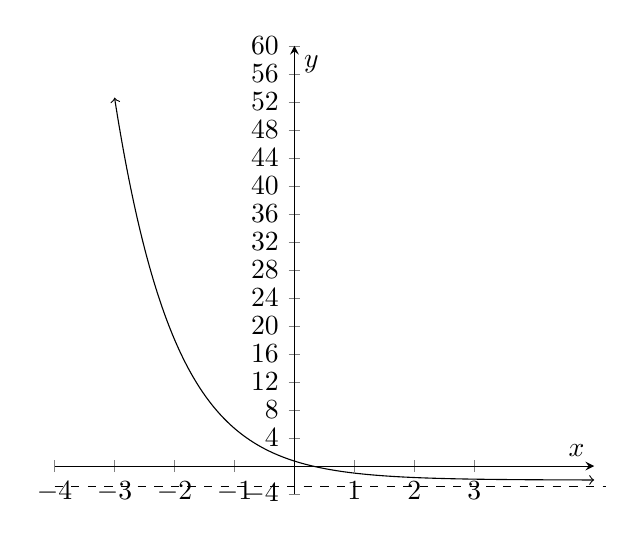
\begin{tikzpicture}
            \begin{axis}[
                axis x line=middle, 
                axis y line=middle, 
                xlabel={$x$}, 
                ylabel={$y$}, 
                xtick={-5,-4,...,3},
                ytick={-4,0,...,60},
                xmin=-4, 
                xmax=5, 
                ymin=-4, 
                ymax=60
                ]
                \addplot[<->,domain=-3:5, samples=300]{e^(-x+1) -2};
            \end{axis}
            \draw[dashed] (0,0.1) -- (7,0.1);
        \end{tikzpicture}
    \end{center}
    
    What is the best parent function for the graph?
    
    \begin{multipleChoice}
        \choice{$f(x)=x$}
        \choice{$f(x)=x^2$}
        \choice{$f(x)=x^3$}
        \choice{$f(x)=\sqrt{x}$}
        \choice[correct]{$f(x)=e^x$}
        \choice{$f(x)=\ln(x)$}
        \choice{$f(x)=|x|$}
    \end{multipleChoice}
    
    \begin{feedback}
        Recall that a key aspect of the various parent functions are the asymptotes. In particular, logarithmic functions have vertical asymptotes whereas exponential functions have horizontal asymptotes. The rest of the functions lack asymptotes entirely.
    \end{feedback}
        
\end{problem}
        
        
        
\begin{problem}
    Consider the following graph:
    \begin{center}
        \begin{tikzpicture}
            \begin{axis}[
                axis x line=middle, 
                axis y line=middle, 
                xlabel={$x$}, 
                ylabel={$y$}, 
                xtick={-8,-6,...,2},
                ytick={0,1,...,4},
                xmin=-8, 
                xmax=2, 
                ymin=-1, 
                ymax=5
                ]
                \addplot[<-,domain=-7:-2, samples=300]{sqrt(-x-2)+1};
            \end{axis}
        \end{tikzpicture}
    \end{center}
    
    What is the best parent function for the graph?
    
    \begin{multipleChoice}
        \choice{$f(x)=x$}
        \choice{$f(x)=x^2$}
        \choice{$f(x)=x^3$}
        \choice[correct]{$f(x)=\sqrt{x}$}
        \choice{$f(x)=e^x$}
        \choice{$f(x)=\ln(x)$}
        \choice{$f(x)=|x|$}
    \end{multipleChoice}
    
    
    \begin{feedback}
        The key feature here is that the function simply ``ends'' at a distinct point on the graph. There is no asymptotic behavior (like with a logarithmic function) nor is there any mirrored or symmetric behavior (like with a parabola or absolute value).
    \end{feedback}
    \begin{feedback}[correct]
        We can tell this graph has a parent function of $\sqrt{x}$ because of the distinctive originating point. All the other parent functions continue to infinity on both sides; either going infinitely left/right (like the polynomial or exponential parent functions) or upward/downward on one side (like with the asymptotic behavior of the logarithm). The square root is the only one of our parent functions that simply ``stops'' at a specific point on one side.
    \end{feedback}
    
\end{problem}
        
        
                
        
\end{document}